% \documentclass[linenumber]{rapidsart}
\documentclass {rapidsart}


\volume{0}
\issue{0}
\pubmonth{June}
\pubyear{2026}
\articletype{research-article}
\doi{0000}
\firstpage{1}
\lastpage{6}

\theoremstyle{plain}
\newtheorem{thm}{Theorem}
\newtheorem{lemma}{Lemma}

\theoremstyle{remark}
\newtheorem{remark}{Remark}
\theoremstyle{definition}
\newtheorem{defin}{Definition}
\hyphenation{de-si-de-rium}
\renewcommand{\thesection}{\arabic{section}}

\usepackage{multirow}
\usepackage{indentfirst}
\usepackage{float}
\usepackage{enumitem}
\usepackage[indonesian]{babel}
\usepackage{natbib}
\usepackage{graphicx}

% \usepackage{apacite}

\begin{document}

\begin{frontmatter}

\title{Deteksi Tindakan Kecurangan Pada Ujian Daring Menggunakan Multimodal Data Berbasis \textit{Deep Learning}}
\runtitle{Deteksi Tindakan Kecurangan Pada Ujian Daring}

\author[1]{\inits{S.S.}\fnms{Valentino} \snm{Prasetyo Putra}
\thanksref{c1}
\ead{valentino.22002@mhs.unesa.ac.id}}

\author[2]{\inits{E.M.}\fnms{Elly Matul} \snm{Imah}}

\thankstext[type=corresp,id=c1]{Corresponding author.}

\address[1]{
\institution{Program Studi S1 Sains Data, Fakultas Matematika dan Ilmu Pengetahuan Alam, Universitas Negeri Surabaya},
\cny{Indonesia}
}
\address[2]{
\institution{Program Studi S1 Kecerdasan Artifisial, Fakultas Matematika dan Ilmu Pengetahuan Alam, Universitas Negeri Surabaya},
\cny{Indonesia}
}

\begin{abstrak}
    Pelaksanaan ujian daring menghadapi berbagai tantangan, salah satunya adalah potensi terjadinya kecurangan akibat keterbatasan pengawasan secara langsung. Penelitian ini mengusulkan pendekatan multimodal berbasis \textit{deep learning} untuk mendeteksi perilaku kecurangan selama ujian daring dengan memanfaatkan data video \textit{wearcam} dan audio yang berasal dari \textit{Online Exam Proctoring} (OEP) Dataset. Pada modalitas video, fitur diekstraksi menggunakan \textit{ResNet50}, \textit{ResNet50V2}, dan \textit{InceptionV3}, kemudian diproses lebih lanjut oleh \textit{LSTM}, \textit{BiLSTM}, dan \textit{GRU} sebagai model klasifikasi. Sementara itu, pada modalitas audio digunakan fitur \textit{Mel-Frequency Cepstral Coefficients} (MFCC) dan \textit{Wavelet} yang diklasifikasikan dengan arsitektur yang sama. Untuk meningkatkan performa prediksi, hasil klasifikasi dari kedua modalitas dikombinasikan melalui metode \textit{ensemble learning} menggunakan pendekatan \textit{weighted soft voting}. Berdasarkan hasil pengujian, kombinasi bobot video dan audio sebesar 0,4:0,6 pada metode \textit{weighted soft voting} memberikan kinerja terbaik untuk klasifikasi biner dengan nilai \textit{accuracy} sebesar 0,97 dan rata-rata \textit{F1-score} sebesar 0,97. Pada skenario klasifikasi multikelas yang terdiri atas enam kategori, pendekatan \textit{ensemble learning} menghasilkan \textit{accuracy} sebesar 0,95 serta rata-rata \textit{F1-score} sebesar 0,91. Temuan penelitian ini menunjukkan bahwa pemanfaatan informasi visual dan audio secara bersamaan mampu memberikan performa deteksi kecurangan yang lebih baik dibandingkan penggunaan satu modalitas saja.
\end{abstrak}



\begin{kunciwords} % Alphabetical; not to repeat anything in the title 
    \kwd{deteksi kecurangan}
    \kwd{multimodal}
    \kwd{\textit{deep learning}}
    \kwd{\textit{ensemble learning}}
    \kwd{\textit{weighted soft voting}}
\end{kunciwords}

\begin{abstract}
    Online examinations face various challenges, one of which is the potential for cheating due to the lack of direct supervision. This study proposes a multimodal deep learning-based approach to detect cheating behavior during online examinations by utilizing wearcam video and audio data from the Online Exam Proctoring (OEP) Dataset. For the video modality, features are extracted using ResNet50, ResNet50V2, and InceptionV3, and subsequently classified using LSTM, BiLSTM, and GRU architectures. For the audio modality, Mel-Frequency Cepstral Coefficients (MFCC) and Wavelet features are extracted and classified using the same architectures. To improve prediction performance, the outputs from both modalities are combined through an ensemble learning approach using weighted soft voting. Experimental results show that the weighted soft voting method with video and audio weights of 0.4 and 0.6, respectively, achieves the best performance for binary classification, obtaining an accuracy of 0.97 and an average F1-score of 0.97. For the six-class classification scenario, the proposed ensemble learning approach achieves an accuracy of 0.95 and an average F1-score of 0.91. These findings demonstrate that the integration of visual and audio information can enhance the detection and classification of cheating behaviors in online examinations compared to the use of a single modality.
\end{abstract}

\begin{keywords} % Alphabetical; not to repeat anything in the title 
\kwd{cheating detection}
\kwd{multimodal learning}
\kwd{deep learning}
\kwd{ensemble learning}
\kwd{weighted soft voting}
\end{keywords}


\received{\today}
\revised{\today}
\accepted{\today}

\end{frontmatter}

\section{Pendahuluan}
\begin{sloppypar}

    Perkembangan teknologi mendorong kemajuan metode dan media pembelajaran \citep{Lindn2023}, baik yang dilakukan secara daring maupun luring, yang kini diadopsi oleh institusi formal maupun layanan pendidikan non-formal seperti kursus daring. Kemudahan akses, fleksibilitas, serta keberagaman materi menjadikan pembelajaran daring semakin diminati \citep{FelipeChild2023,Turan2022}. Dalam proses pembelajaran, evaluasi melalui ujian masih banyak digunakan sebagai sarana utama untuk mengukur pemahaman dan kompetensi peserta didik \citep{Ababneh2022}. Integritas ujian daring memiliki tantangan tersendiri karena pengawasan tidak dapat dilakukan secara langsung sehingga ruang terjadinya kecurangan jauh lebih besar dibandingkan ujian luring \citep{Fendler2024}. \citet{Newton2024} menunjukkan bahwa praktik kecurangan terjadi dalam skala signifikan, dengan lebih dari 44,7\% mahasiswa mengaku pernah melakukannya dan angkanya meningkat selama periode pandemi. Kondisi ini menegaskan perlunya sistem pemantauan yang mampu mendeteksi perilaku kecurangan secara otomatis dalam ujian daring \citep{Sakhipov2025}.
    
    Berbagai penelitian telah mengusulkan pendekatan untuk deteksi kecurangan berbasis \textit{deep learning}. \citet{Kaddoura2022} mengembangkan sistem multimodal yang memanfaatkan data visual dan audio untuk mendeteksi perilaku mencurigakan selama ujian daring. Pendekatan serupa juga dikembangkan oleh \citet{SangeetaLamba2024}, yang mengintegrasikan deteksi wajah, aktivitas suara, serta analisis arah pandangan dan pose kepala menggunakan arsitektur CNN dan BiLSTM untuk menghasilkan prediksi kecurangan yang lebih komprehensif. \citet{SihamEssahraui2025} berfokus pada analisis citra atau video menggunakan model berbasis \textit{Convolutional Neural Network} (CNN) seperti ResNet50, MobileNetV2, dan EfficientNet serta metode deteksi objek. Pendekatan berbasis \textit{machine learning} konvensional seperti \textit{Support Vector Machine} (SVM), \textit{Decision Tree}, dan XGBoost juga telah dieksplorasi untuk memprediksi perilaku curang pada ujian digital \citep{Erdem2025}. Penelitian yang dilakukan oleh \citet{Smirani2022} mengembangkan sistem deteksi kecurangan berbasis CNN yang menganalisis aktivitas peserta ujian melalui tangkapan layar komputer, pola navigasi, dan alamat IP tanpa menggunakan kamera. Meskipun pendekatan-pendekatan tersebut menunjukkan performa yang menjanjikan dalam membedakan perilaku peserta ujian secara umum, sebagian besar penelitian masih menerapkan skema \textit{binary classification} yang hanya menghasilkan label `curang'' dan `tidak curang''.
    
    Pendekatan \textit{binary classification} ini memiliki keterbatasan dalam konteks ujian daring yang kompleks. Pertama, model tidak mampu membedakan jenis atau bentuk kecurangan yang dilakukan, sehingga berbagai perilaku seperti melihat catatan, membuka laman internet, atau menggunakan perangkat lain diperlakukan sebagai satu kategori yang sama \citep{Erdem2025,Henderson2023}. Kedua, keterbatasan ini menghambat analisis perilaku secara lebih mendalam karena sistem tidak menyediakan informasi detail mengenai pola dan tingkat pelanggaran yang terjadi. Akibatnya, keluaran sistem menjadi kurang informatif dan belum optimal untuk mendukung pengambilan keputusan oleh pengawas maupun institusi pendidikan, seperti penentuan sanksi, evaluasi kebijakan pengawasan, maupun strategi pencegahan kecurangan yang lebih tepat sasaran.
    
    Sebagai respons terhadap keterbatasan tersebut, beberapa penelitian mulai mengembangkan arsitektur yang lebih kompleks, seperti \textit{framework} berbasis \textit{spatio-temporal graph} untuk mengintegrasikan fitur postur tubuh, latar belakang, dan atribut wajah guna meningkatkan akurasi deteksi \citep{Liu2024}. Pemanfaatan model pralatih (\textit{transfer learning}) juga telah menjadi strategi penting untuk meningkatkan performa pada dataset terbatas, meskipun memerlukan strategi \textit{fine-tuning} yang tepat agar tidak terjadi \textit{overfitting} \citep{Becherer2019}. Berbagai arsitektur CNN modern, seperti ResNet50V2 dan InceptionV3, telah banyak dimanfaatkan sebagai \textit{feature extractor} pada tugas pengenalan citra dan video. ResNet50V2 menggunakan skema \textit{pre-activation residual block} yang membantu menjaga stabilitas pelatihan pada jaringan yang dalam \citep{He2016}, sedangkan InceptionV3 menerapkan ekstraksi fitur multiskala melalui kombinasi konvolusi paralel dengan ukuran kernel berbeda \citep{Hassan2025,Sharma2022}.
    
    Berangkat dari perkembangan tersebut, penelitian ini mengembangkan sistem pengawas ujian daring berbasis \textit{computer vision} dengan pendekatan \textit{ensemble machine learning}. Sistem memanfaatkan kamera \textit{wearable} berbentuk kacamata (\textit{wearcam}) untuk menangkap sudut pandang pengguna secara langsung sehingga aktivitas seperti membaca buku atau penggunaan perangkat lain dapat teridentifikasi secara visual \citep{Thomas2022}. Pada tahap pertama dilakukan klasifikasi biner untuk membedakan perilaku tidak curang dan curang menggunakan dua modalitas, yaitu video \textit{wearcam} dan audio. Hasil prediksi dari kedua modalitas kemudian digabungkan menggunakan metode \textit{weighted soft voting} untuk menghasilkan keputusan biner yang lebih \textit{robust}. Hanya sampel yang terdeteksi sebagai curang yang diproses pada tahap kedua untuk diklasifikasikan ke dalam lima jenis perilaku kecurangan. Pendekatan \textit{ensemble machine learning} dengan pembagian tahap seperti ini masih jarang diterapkan pada penelitian sebelumnya. Dengan demikian, penelitian ini tidak hanya meningkatkan ketelitian deteksi, tetapi juga memberikan informasi yang lebih spesifik mengenai jenis kecurangan yang terjadi. Seluruh alur penelitian ditunjukkan pada Gambar~\ref{fig:arsitektur_sistem}.

\begin{figure}[htbp]
    \centering
    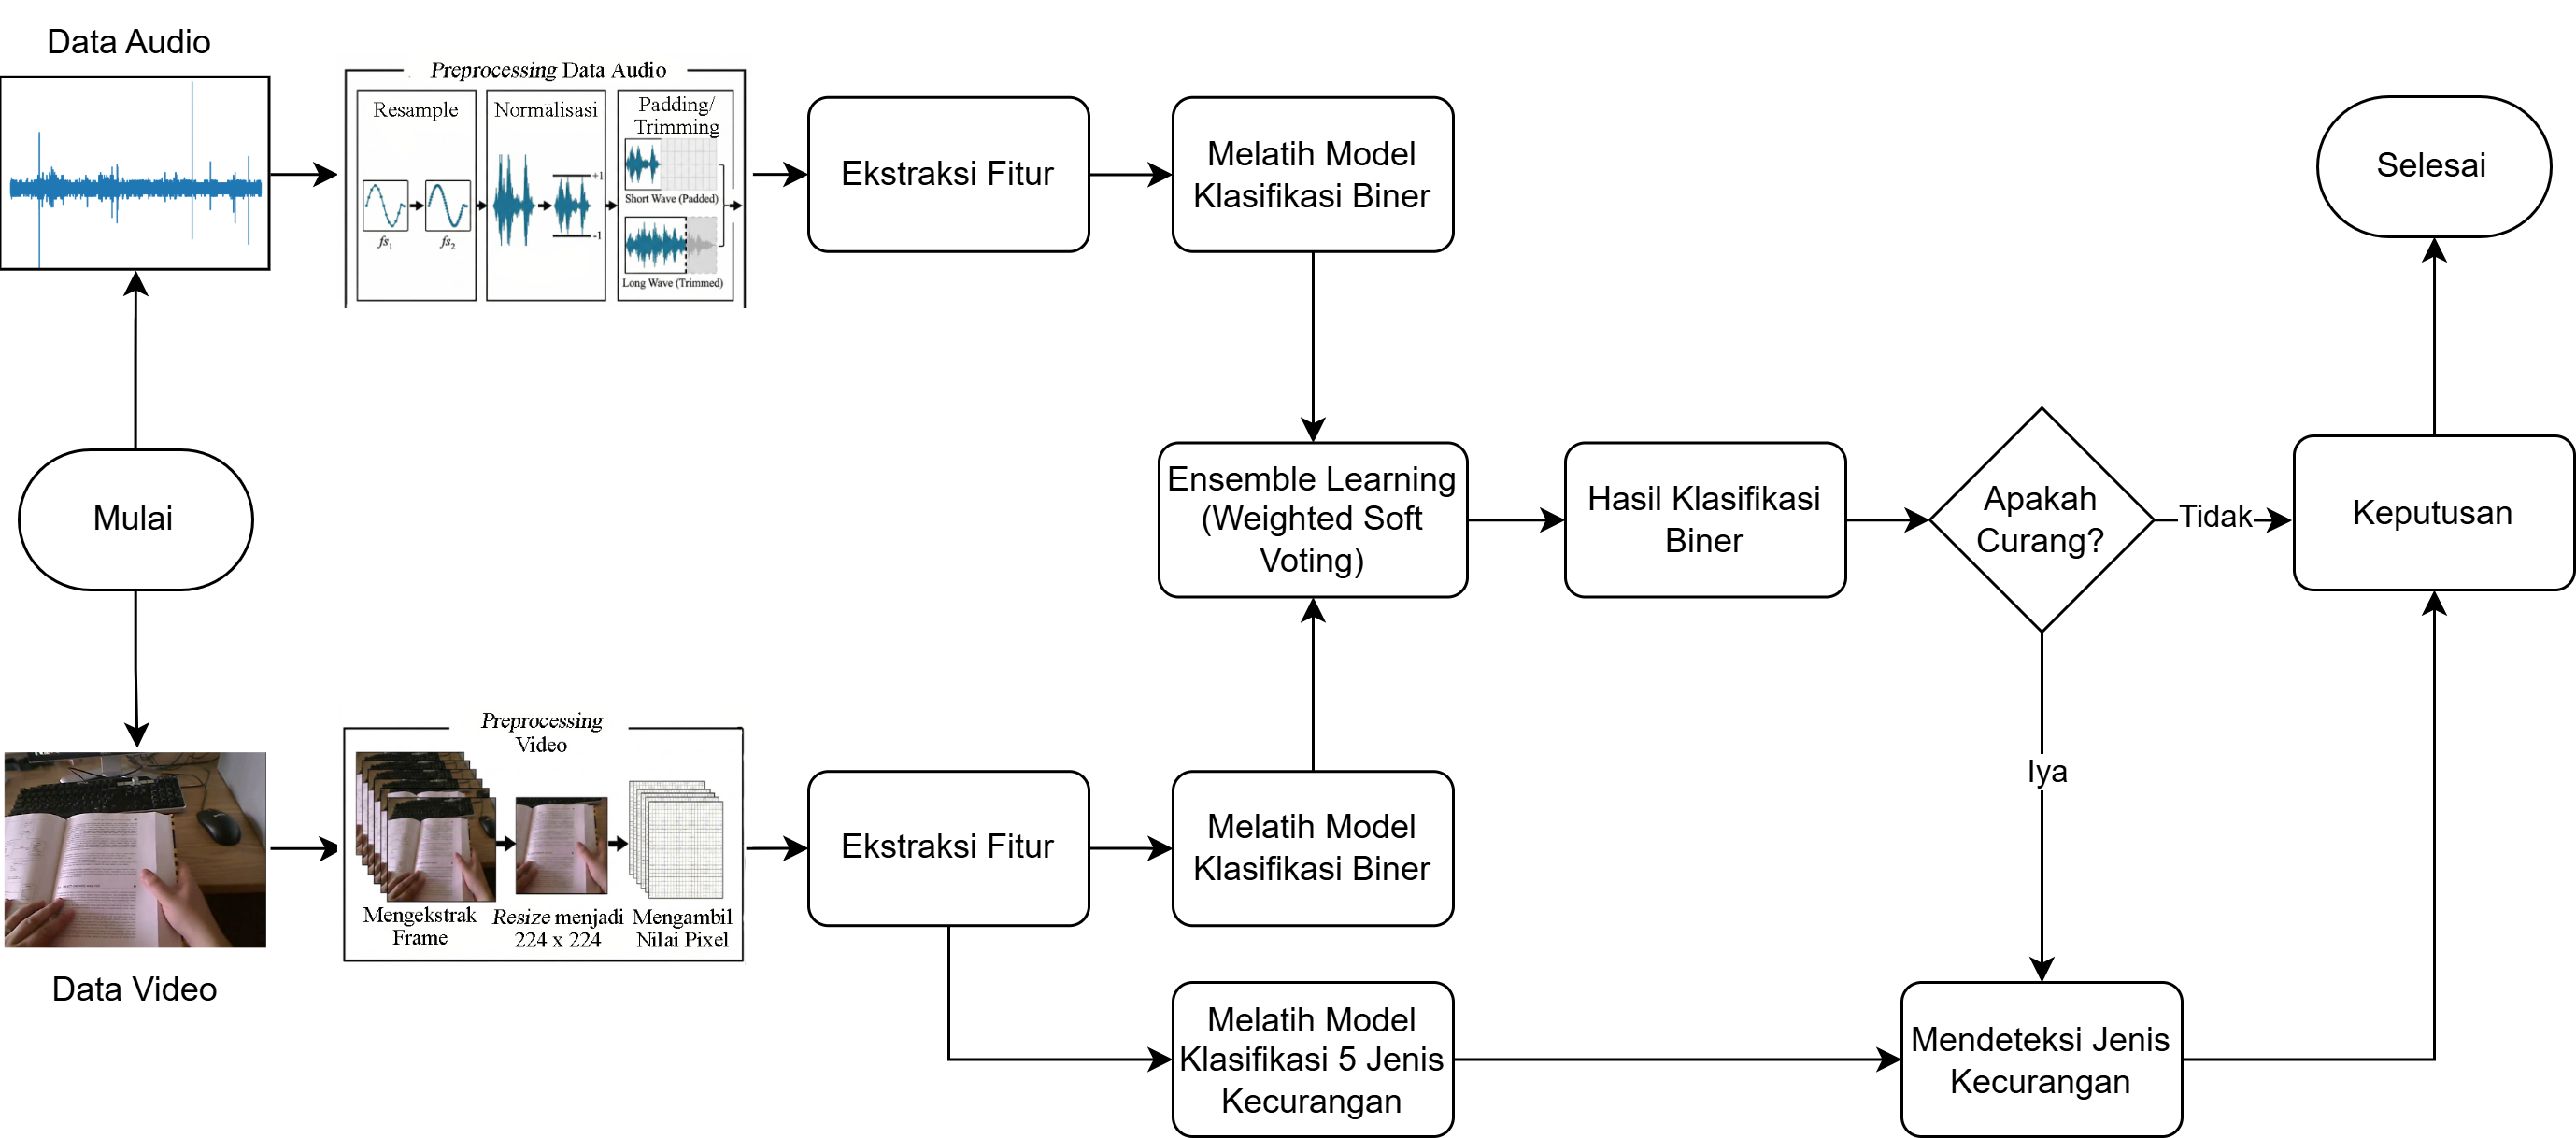
\includegraphics[width=0.9\textwidth]{Figure/alur_penelitian.png}
    \caption{Diagram Alur Rancangan Penelitian}
    \label{fig:arsitektur_sistem}
\end{figure}

\end{sloppypar}


\section{Metode}
\subsection{Dataset}
    Data yang digunakan dalam penelitian ini merupakan data sekunder yang berasal dari \textit{Online Exam Proctoring} (OEP) Dataset yang dikembangkan oleh \textit{Computer Vision Laboratory}, \textit{Michigan State University} (MSU) \citep{Atoum2017}. Dataset ini dirancang untuk penelitian deteksi kecurangan pada ujian daring dan berisi rekaman audio serta video dari 24 peserta. Sebanyak 15 peserta mensimulasikan berbagai perilaku kecurangan, sedangkan 9 peserta lainnya mengikuti ujian dengan skenario kecurangan yang dipicu oleh pengawas. Dataset menyediakan beberapa kanal rekaman, yaitu video kamera depan, video \textit{wearable camera} (\textit{wearcam}), dan audio. Penelitian ini memanfaatkan data video \textit{wearcam} dan audio karena kedua modalitas tersebut mampu merepresentasikan aktivitas lingkungan serta indikasi kecurangan yang tidak selalu dapat diamati melalui informasi visual saja.
    
\begin{figure}[htbp]
    \centering
    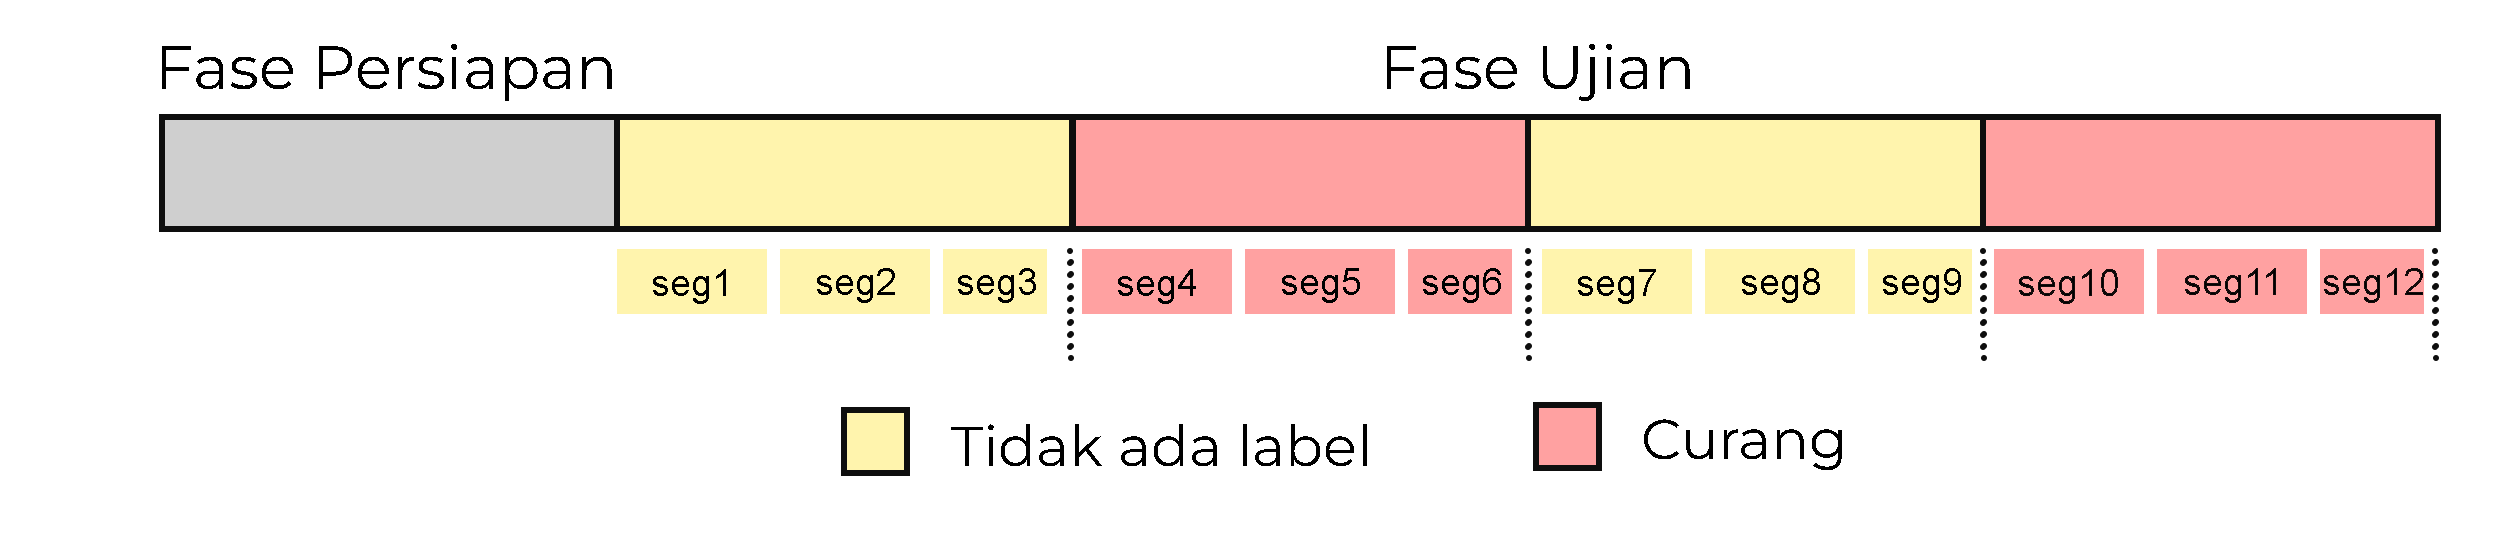
\includegraphics[width=0.9\textwidth]{Figure/anotasi.png}
    \caption{Proses Anotasi Label Tidak Curang Data Video}
    \label{fig:anotasi_tidak_curang}
\end{figure}

    Selain label kecurangan yang telah tersedia pada dataset, penelitian ini menambahkan label tidak curang melalui proses anotasi manual untuk merepresentasikan aktivitas normal selama ujian. Proses anotasi label tidak curang ditunjukkan pada Gambar~\ref{fig:anotasi_tidak_curang} dan hanya dilakukan pada segmen waktu yang tidak memiliki label pada \textit{ground truth} serta tidak menunjukkan indikasi kecurangan berdasarkan hasil pemeriksaan visual. Pendekatan pelabelan selektif ini bertujuan untuk mengurangi kesalahan pelabelan dan meningkatkan keandalan model dalam membedakan kondisi curang dan tidak curang. Distribusi jumlah data untuk setiap label ditampilkan pada Tabel~\ref{tab:distribusi_label}.

\begin{table}[htbp]
\caption{Distribusi per label}
\label{tab:distribusi_label}
\centering
\begin{tabular*}{0.6\textwidth}{@{\extracolsep{\fill}}lc@{}}
\hline
\textbf{Label} & \textbf{Jumlah} \\
\hline
Tidak curang & 988 \\
Membaca buku & 192 \\
Berbicara dengan orang lain & 285 \\
Menggunakan internet & 52 \\
Menelpon teman & 15 \\
Menggunakan ponsel & 20 \\
\hline
\end{tabular*}
\end{table}



\subsection{Pemrosesan Data}
\subsubsection{Prapemrosesan Data Video}

Tahap prapemrosesan dilakukan untuk memastikan bahwa data video memiliki format dan struktur yang konsisten sebelum memasuki tahap ekstraksi fitur dan klasifikasi. Seluruh video terlebih dahulu dikelompokkan berdasarkan kelasnya, kemudian sistem membaca setiap video dan memeriksa jumlah \textit{frame} yang tersedia. Video yang memiliki jumlah \textit{frame} kurang dari 25 \textit{frame} dieliminasi untuk menjaga konsistensi antar sampel serta mengurangi potensi ketidakseimbangan data.

Video yang memenuhi kriteria kemudian diambil sebanyak 25 \textit{frame} yang tersebar secara merata dari awal hingga akhir durasi rekaman. Pendekatan ini memungkinkan setiap video memiliki representasi visual yang proporsional terhadap keseluruhan aktivitas tanpa perlu memproses seluruh \textit{frame}, sehingga dapat meningkatkan efisiensi komputasi \citep{Shen2025}. Setiap \textit{frame} yang terpilih kemudian diubah ukurannya menjadi 224 $\times$ 224 piksel agar seluruh citra memiliki dimensi yang seragam. Hasil dari tahap prapemrosesan ini berupa struktur data berdimensi $(n, 25, 224, 224, 3)$, dengan $n$ menyatakan jumlah video yang digunakan dalam dataset.

\subsubsection{Prapemrosesan Data Audio}

Tahapan prapemrosesan dimulai dengan membaca seluruh berkas audio dari setiap kelas dan melakukan validasi untuk memastikan tidak terdapat berkas yang kosong atau rusak. Audio yang tidak memenuhi kriteria kualitas dikeluarkan dari proses pengolahan agar konsistensi data tetap terjaga. Seluruh audio kemudian dikonversi ke format yang seragam dengan frekuensi sampel tetap untuk menyamakan resolusi temporal antar sampel serta mengurangi variasi yang disebabkan oleh perbedaan perangkat perekaman.

Setiap sinyal audio selanjutnya dinormalisasi untuk menyeimbangkan amplitudo sehingga perbedaan intensitas suara tidak memengaruhi proses pelatihan model. Panjang sinyal juga diseragamkan melalui proses pemotongan atau penambahan \textit{padding} agar seluruh sampel memiliki jumlah \textit{frame} waktu yang sama. Proses ini dilakukan untuk memastikan bahwa setiap sampel sesuai dengan kebutuhan masukan berdimensi tetap pada model klasifikasi.


\subsection{Ekstraksi Fitur}
\subsubsection{Ekstraksi Fitur Data Video Menggunakan ResNet50}

\begin{figure}[htbp]
    \centering
    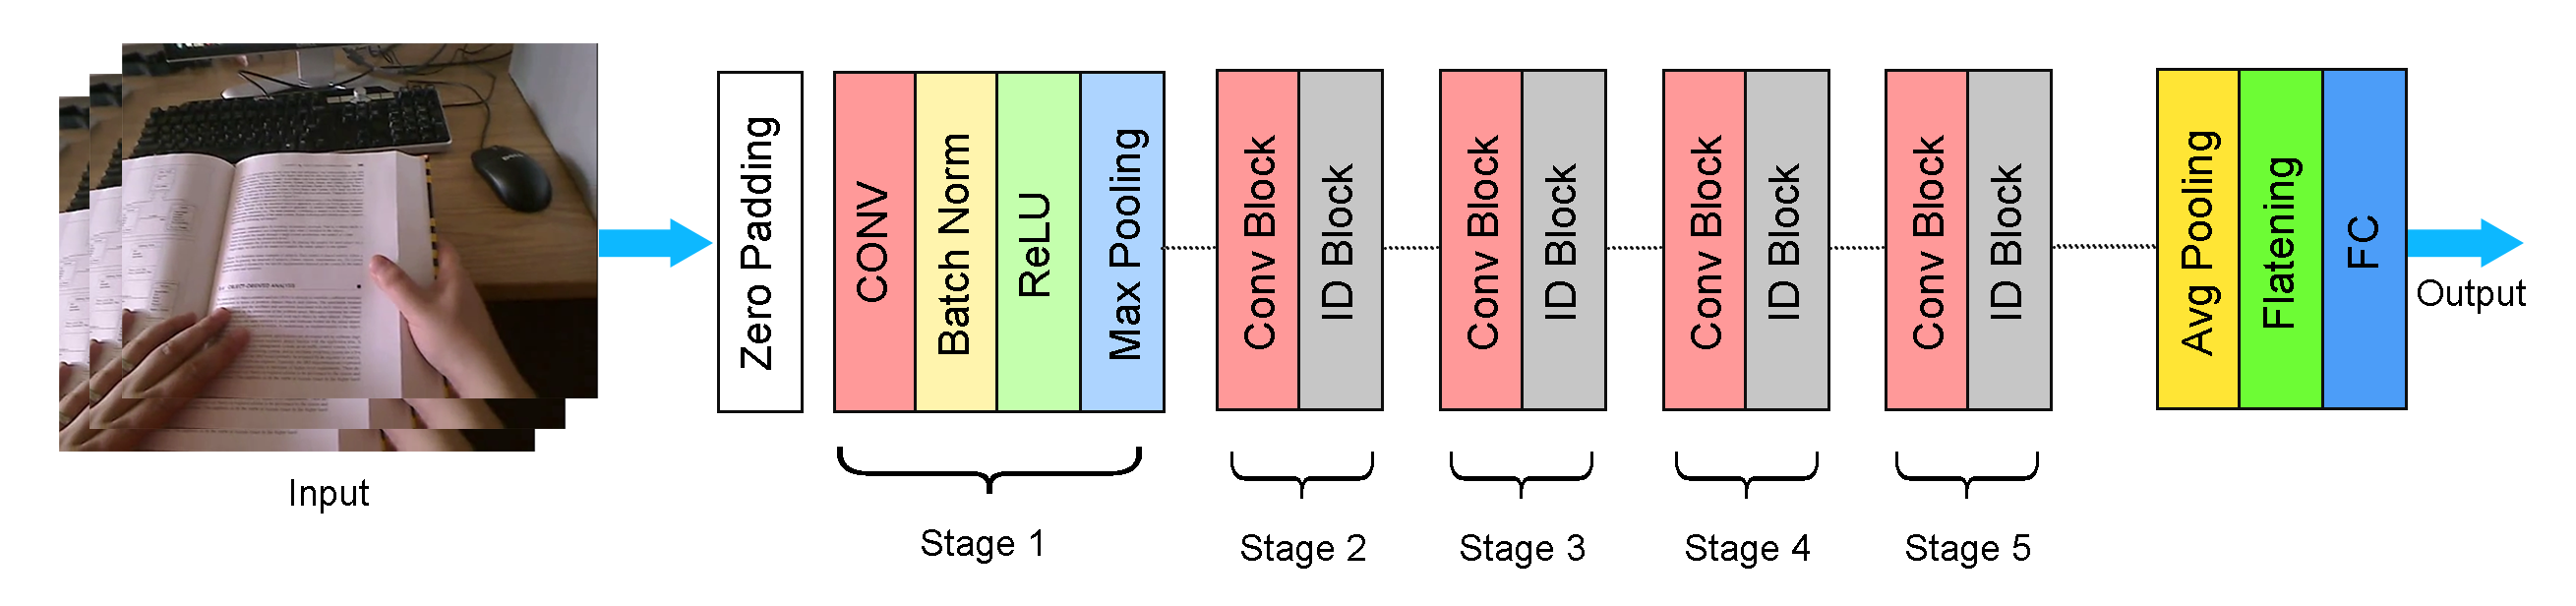
\includegraphics[width=0.9\linewidth]{Figure/Resnet50.png}
    \caption{Arsitektur ResNet50}
    \label{fig:arsitektur-resnet50}
\end{figure}

ResNet50 menggunakan mekanisme \textit{residual learning} melalui \textit{skip connection} untuk meningkatkan stabilitas pelatihan jaringan yang dalam serta mengurangi permasalahan \textit{vanishing gradient}, sehingga efektif dalam mengekstraksi fitur visual tingkat tinggi dari citra \citep{Sharma2022}. Arsitektur ResNet50 terdiri atas beberapa \textit{residual stage} yang dimulai dari lapisan konvolusi awal hingga \textit{fully connected layer}, sebagaimana ditunjukkan pada Gambar~\ref{fig:arsitektur-resnet50}. Secara matematis, jika $x$ merupakan masukan suatu blok residual dan $F(x)$ adalah fungsi transformasi nonlinier yang terdiri atas operasi konvolusi, \textit{batch normalization}, dan fungsi aktivasi, maka keluaran blok residual dapat dirumuskan sebagai berikut:

\begin{equation}
H(x) = F(x) + x
\label{eq}
\end{equation}

Penjumlahan antara $F(x)$ dan $x$ membentuk \textit{identity mapping} yang memungkinkan jaringan mempelajari fungsi residual secara langsung sehingga mempermudah proses optimisasi pada jaringan yang sangat dalam. Pada proses \textit{backpropagation}, jika $L$ menyatakan fungsi \textit{loss}, maka gradien terhadap masukan $x$ dirumuskan sebagai berikut:

\begin{equation}
\frac{\partial L}{\partial x}
=
\frac{\partial L}{\partial H}
\left(
\frac{\partial F(x)}{\partial x}
+
1
\right)
\label{eq:residual_gradient}
\end{equation}

Suku $+1$ berasal dari jalur identitas sehingga gradien tetap dapat mengalir ke lapisan sebelumnya meskipun nilai $\frac{\partial F(x)}{\partial x}$ sangat kecil. Melalui mekanisme tersebut, ResNet50 mampu mengurangi degradasi kinerja pada jaringan yang dalam dan efektif digunakan sebagai model ekstraksi fitur pada tugas klasifikasi citra berbasis \textit{deep learning}.

\subsubsection{Ekstraksi Fitur Data Audio Menggunakan \textit{Mel-Frequency Cepstral Coefficients} (MFCC)}

\begin{figure}[htbp]
    \centering
    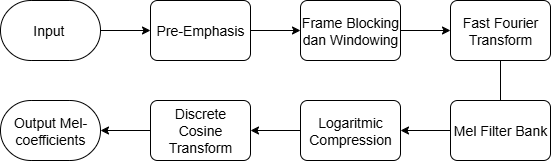
\includegraphics[width=0.9\linewidth]{Figure/mfcc.png}
    \caption{Alur MFCC}
    \label{fig:mfcc}
\end{figure}

\textit{Mel-Frequency Cepstral Coefficients} (MFCC) merupakan metode ekstraksi fitur audio yang merepresentasikan karakteristik spektral sinyal berdasarkan persepsi pendengaran manusia dan banyak digunakan pada tugas klasifikasi suara. Dalam konteks pengenalan suara, sinyal audio dapat memuat berbagai informasi seperti identitas, emosi, usia, dan kondisi psikologis seseorang \citep{Ali2021}. Pada Gambar~\ref{fig:mfcc}, proses MFCC diawali dengan tahap \textit{pre-emphasis} untuk memperkuat komponen frekuensi tinggi, yang dirumuskan sebagai berikut:

\begin{equation}
y(n) = x(n) - \alpha x(n-1)
\label{eq}
\end{equation}

Sinyal kemudian dibagi menjadi beberapa \textit{frame} dan diterapkan proses \textit{windowing} untuk mengurangi diskontinuitas antar \textit{frame}. Setiap \textit{frame} selanjutnya ditransformasikan ke domain frekuensi menggunakan \textit{Fast Fourier Transform} (FFT) sebagai berikut:

\begin{equation}
X(k)=\sum_{n=0}^{N-1} x(n)e^{-j\frac{2\pi kn}{N}}
\label{eq}
\end{equation}

Spektrum frekuensi yang dihasilkan kemudian diproses menggunakan \textit{mel filter bank} untuk memperoleh energi pada skala \textit{mel} dan dikonversi ke bentuk logaritmik sebagai berikut:

\begin{equation}
S_m = \log(E_m)
\label{eq}
\end{equation}

Tahap akhir adalah penerapan \textit{Discrete Cosine Transform} (DCT) untuk menghasilkan koefisien MFCC yang merepresentasikan amplop spektral sinyal secara kompak. Koefisien tersebut digunakan sebagai fitur masukan pada model pembelajaran mesin karena mampu menangkap informasi akustik yang penting secara efisien.


\subsection{Klasifikasi}
\subsubsection{\textit{Bidirectional Long Short-Term Memory} (Bi-LSTM)}

\begin{figure}[htbp]
    \centering
    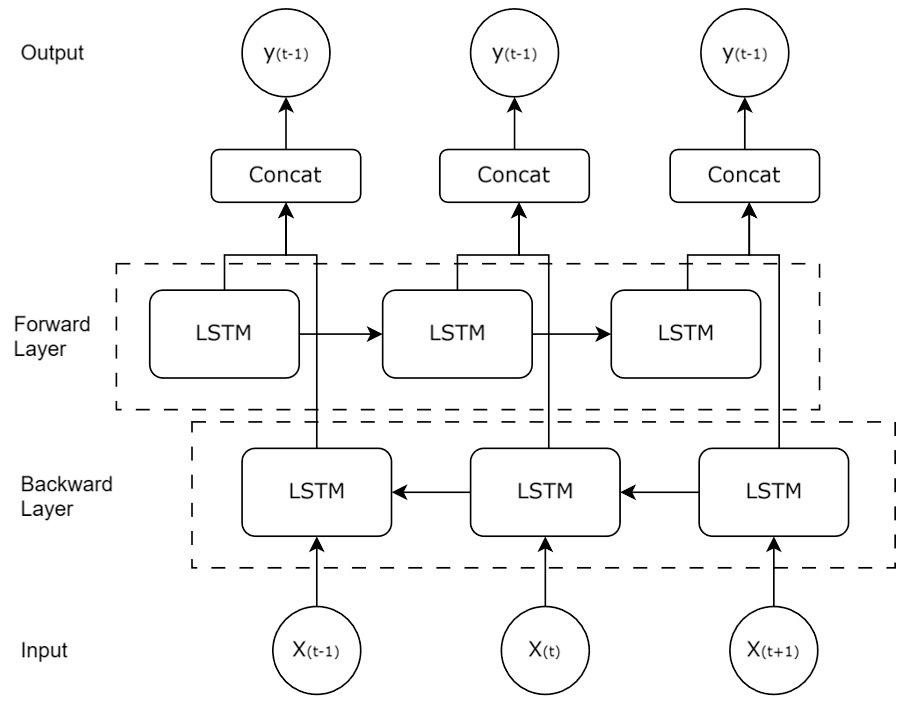
\includegraphics[width=0.5\linewidth]{Figure/BiLSTM.png}
    \caption{Arsitektur BiLSTM}
    \label{fig:arsitektur-bilstm}
\end{figure}

\textit{Bidirectional Long Short-Term Memory} (BiLSTM) merupakan pengembangan dari LSTM yang memproses data sekuensial dalam dua arah, yaitu \textit{forward} dan \textit{backward}. Arsitektur BiLSTM ditunjukkan pada Gambar~\ref{fig:arsitektur-bilstm}. Berbeda dengan LSTM konvensional yang hanya memproses urutan data dalam satu arah, BiLSTM menggabungkan keluaran dari kedua arah untuk membentuk representasi fitur akhir yang dirumuskan sebagai berikut:

\begin{equation}
y(t) = \left[ y_f(t),, y_b(t) \right]
\label{eq}
\end{equation}

Dengan mekanisme tersebut, informasi dari masa lalu maupun masa depan dapat dimanfaatkan secara simultan. Pendekatan ini menghasilkan representasi temporal yang lebih komprehensif dan berpotensi meningkatkan kinerja klasifikasi pada data video yang memiliki dinamika waktu yang kompleks \citep{Liu2024}. Pada penelitian ini, arsitektur BiLSTM terdiri atas dua lapisan BiLSTM dengan fungsi aktivasi \textit{tanh} yang menghasilkan keluaran berdimensi $n \times 25 \times 512$ dan $n \times 256$. Representasi fitur yang diperoleh selanjutnya diproses melalui lapisan \textit{Dense} dengan fungsi aktivasi \textit{ReLU} berukuran $n \times 128$, kemudian dilanjutkan dengan \textit{Batch Normalization} dan \textit{Dropout} untuk meningkatkan stabilitas pelatihan serta mengurangi risiko \textit{overfitting}. Pada lapisan keluaran, digunakan lapisan \textit{Dense} dengan fungsi aktivasi \textit{Softmax} yang menghasilkan keluaran berdimensi $n \times n_{class}$ untuk klasifikasi multikelas, sedangkan pada klasifikasi biner digunakan fungsi aktivasi \textit{sigmoid}.

\subsubsection{\textit{Gated Recurrent Unit} (GRU)}

\begin{figure}[htbp]
    \centering
    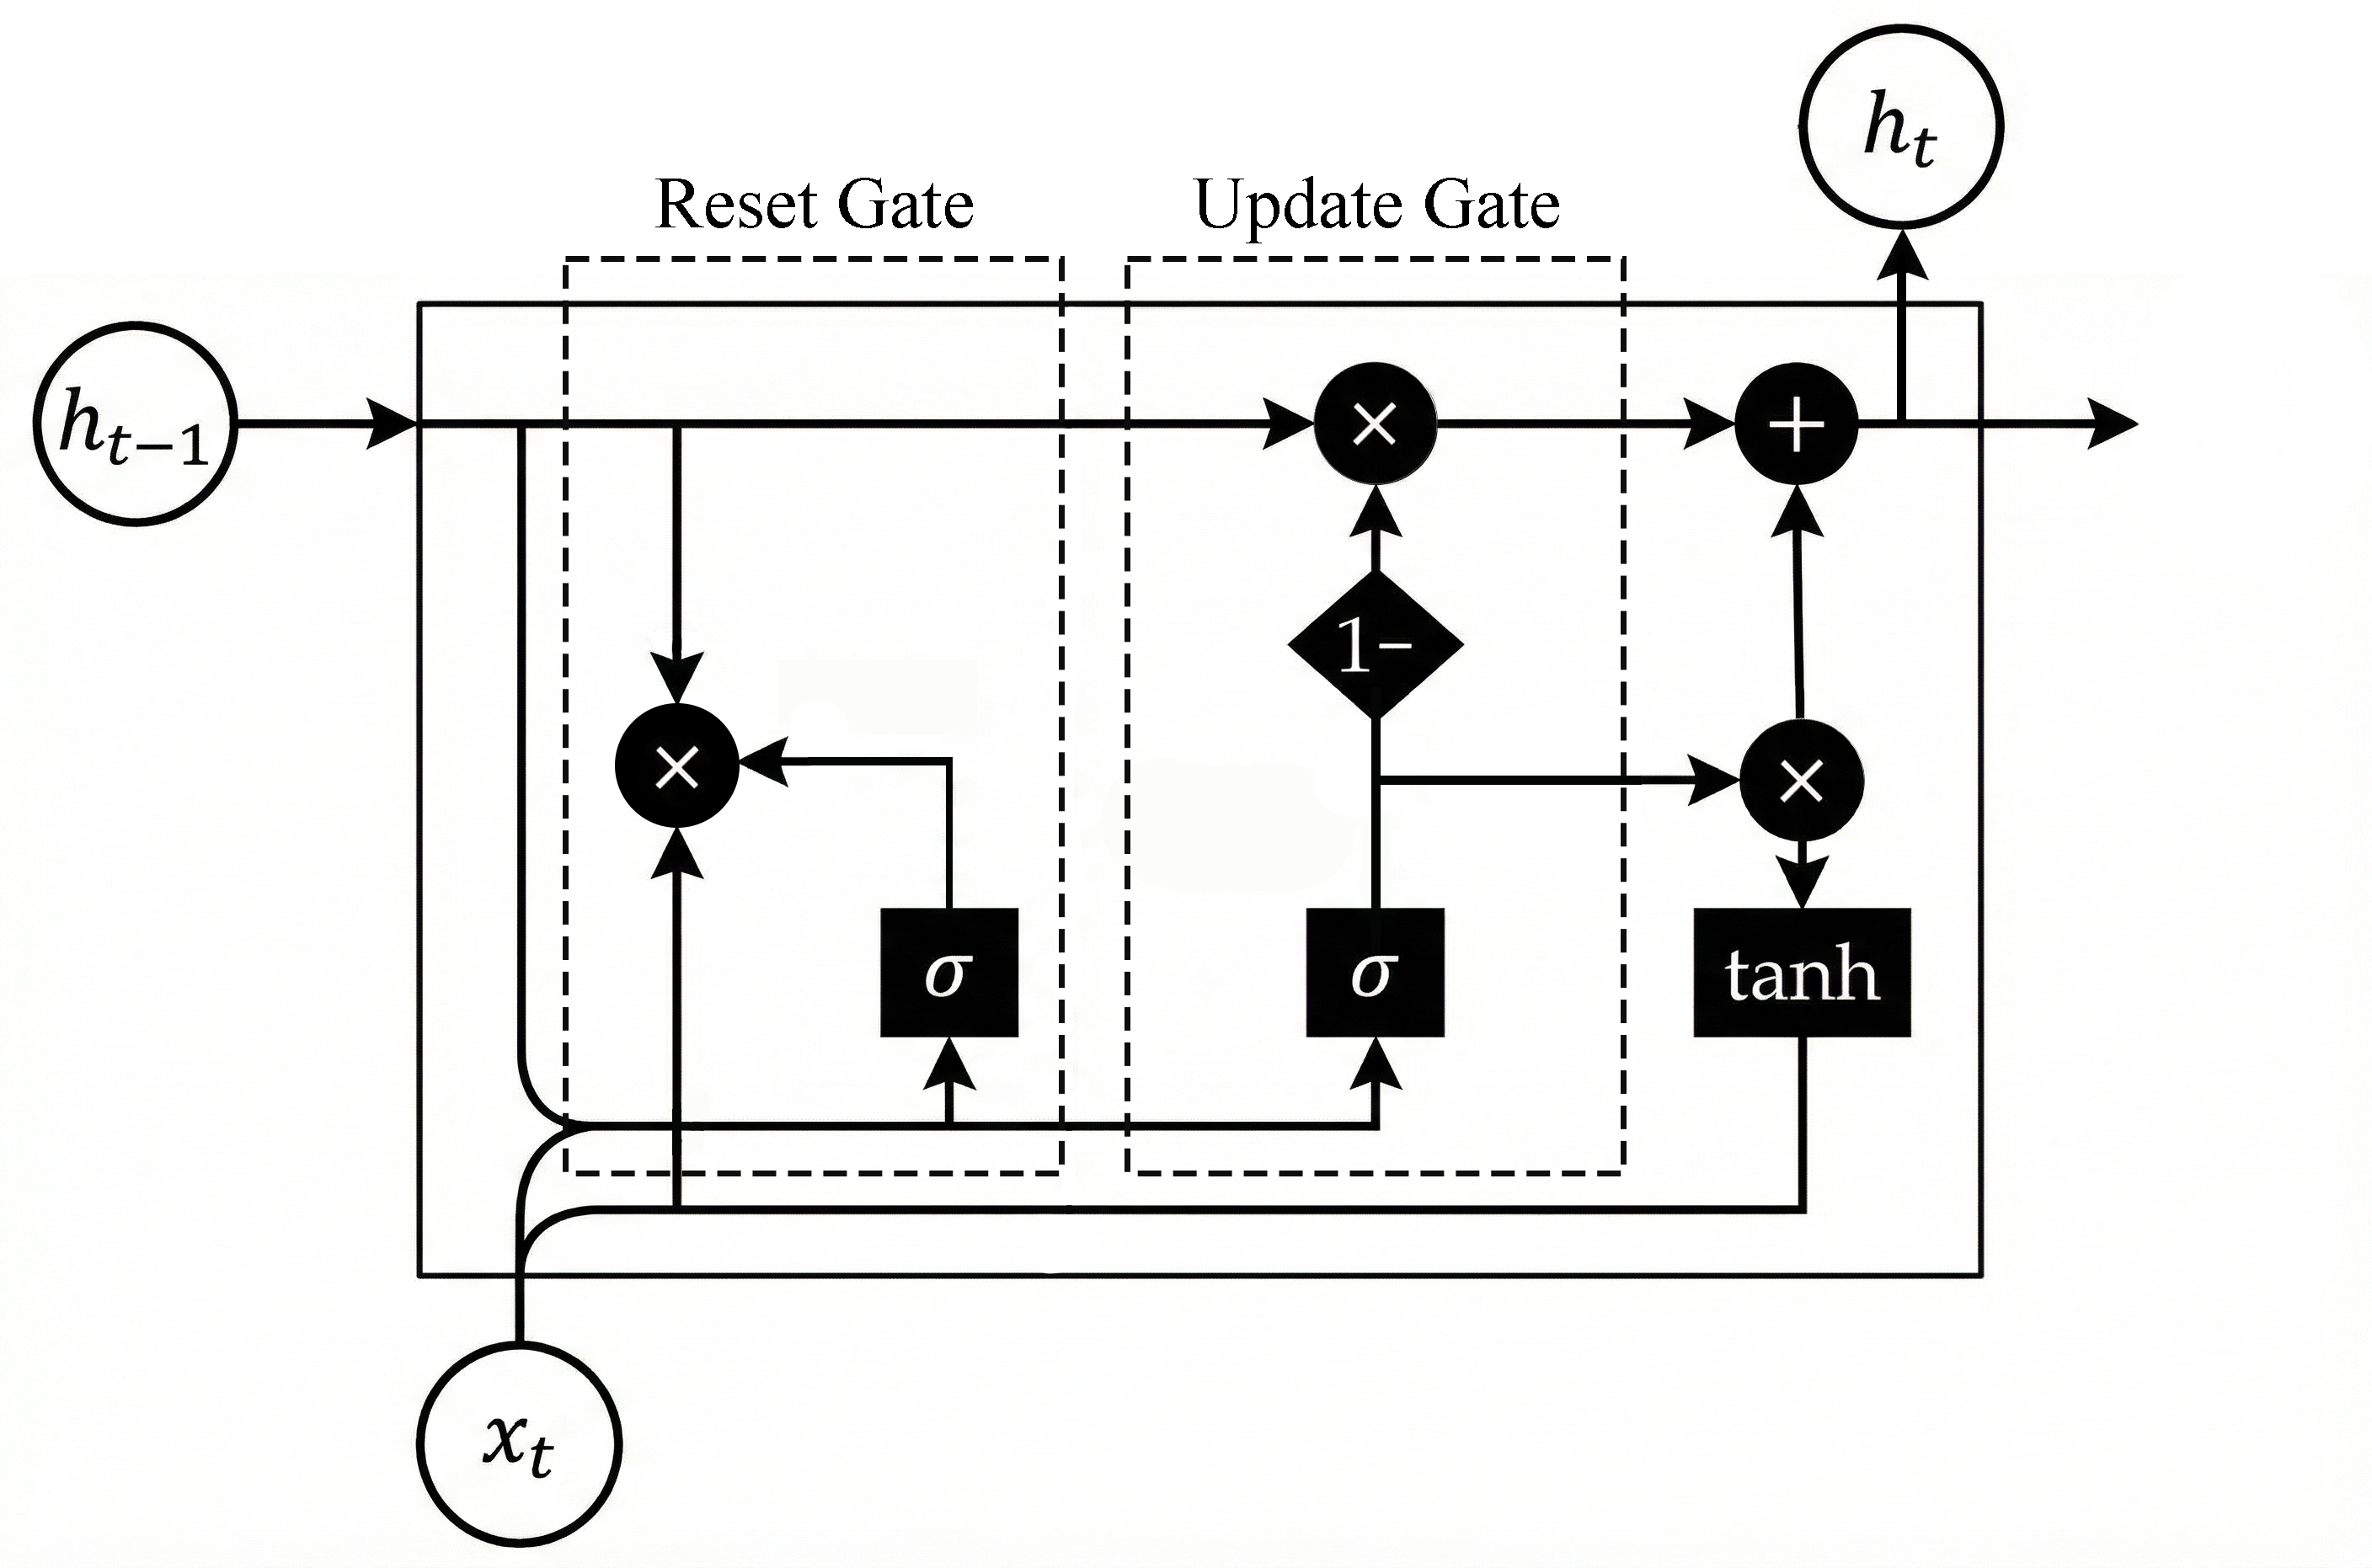
\includegraphics[width=0.5\linewidth]{Figure/GRU.png}
    \caption{Arsitektur GRU}
    \label{fig:arsitektur-gru}
\end{figure}

\textit{Gated Recurrent Unit} (GRU) merupakan varian dari \textit{Recurrent Neural Network} (RNN) yang lebih ringan dibandingkan LSTM karena memiliki jumlah parameter yang lebih sedikit, namun tetap mampu memodelkan dependensi temporal secara efektif \citep{Waqas2024}. GRU menggunakan dua mekanisme utama, yaitu \textit{update gate} dan \textit{reset gate}, sehingga struktur model menjadi lebih sederhana dan proses pelatihan dapat dilakukan dengan lebih efisien. Arsitektur dasar GRU ditunjukkan pada Gambar~\ref{fig:arsitektur-gru}.

Kedua mekanisme tersebut digunakan untuk menghitung kandidat \textit{hidden state} dan memperbarui keadaan memori sebagaimana dirumuskan pada Persamaan~\ref{eq} dan Persamaan~\ref{eq}.

\begin{equation}
\tilde{h}^{(t)}
=
\tanh
\left(
W_h x^{(t)}
+
R_h
\left(
r^{(t)}
\odot
h^{(t-1)}
\right)
+
b_h
\right)
\label{eq:gru_candidate}
\end{equation}

\begin{equation}
h^{(t)}
=
\left(
1-z^{(t)}
\right)
\odot
h^{(t-1)}
+
z^{(t)}
\odot
\tilde{h}^{(t)}
\label{eq:gru_hidden}
\end{equation}

Pada penelitian ini, arsitektur GRU terdiri atas dua lapisan GRU dengan fungsi aktivasi \textit{tanh} yang menghasilkan keluaran berdimensi $n \times 25 \times 256$ dan $n \times 128$. Representasi fitur yang dihasilkan kemudian diproses melalui lapisan \textit{Dense} dengan fungsi aktivasi \textit{ReLU} berukuran $n \times 128$, kemudian dilanjutkan dengan \textit{Batch Normalization} dan \textit{Dropout} untuk meningkatkan stabilitas pelatihan serta mengurangi risiko \textit{overfitting}. Pada lapisan keluaran digunakan lapisan \textit{Dense} dengan fungsi aktivasi \textit{Softmax} yang menghasilkan keluaran berdimensi $n \times n_{class}$ untuk klasifikasi multikelas, sedangkan pada klasifikasi biner digunakan fungsi aktivasi \textit{sigmoid}.

\subsection{\textit{Ensemble Learning (Weighted Soft Voting)}}

Hasil ekstraksi fitur dari data video dan audio selanjutnya diklasifikasikan menggunakan model sekuens berbasis \textit{Recurrent Neural Network} (RNN), yaitu \textit{Bidirectional Long Short-Term Memory} (BiLSTM) dan \textit{Gated Recurrent Unit} (GRU). Kedua model dipilih karena mampu menangani dependensi temporal pada data sekuensial serta memiliki performa yang stabil dibandingkan metode konvensional \citep{Ahmadzadeh2022}.

Dalam penelitian berbasis \textit{multimodal learning}, khususnya yang menggabungkan data visual dan audio, pendekatan \textit{ensemble learning} semakin banyak digunakan sebagai pengembangan dari metode \textit{fusion} konvensional. \textit{Ensemble learning} merujuk pada strategi penggunaan beberapa model secara paralel yang kemudian menggabungkan keluaran masing-masing model untuk memperoleh prediksi akhir yang lebih akurat \citep{Li2021}.

Setiap model pada masing-masing modalitas menghasilkan probabilitas prediksi untuk setiap kelas. Untuk meningkatkan kinerja sistem secara keseluruhan, hasil prediksi dari kedua modalitas kemudian digabungkan menggunakan pendekatan \textit{ensemble learning} pada tingkat keputusan (\textit{decision-level fusion}). Pendekatan ini menawarkan keunggulan berupa modularitas dan fleksibilitas, serta kemampuan dalam memanfaatkan kekuatan setiap modalitas secara optimal sambil mengurangi kelemahan yang umumnya muncul pada model tunggal.

Metode yang digunakan dalam penelitian ini adalah \textit{weighted soft voting}, yang mengombinasikan probabilitas keluaran dari \textit{classifier} video dan audio secara linear berdasarkan bobot kontribusi masing-masing modalitas.

Pada metode ini, probabilitas akhir untuk setiap kelas dihitung menggunakan persamaan berikut:

\begin{equation}
P_{\text{final}}(c)
=
w_v \cdot P_v(c)
+
w_a \cdot P_a(c)
\label{eq:weighted_soft_voting}
\end{equation}

di mana $P_v(c)$ dan $P_a(c)$ masing-masing merupakan probabilitas prediksi dari \textit{classifier} video dan audio terhadap kelas $c$, sedangkan $w_v$ dan $w_a$ merupakan bobot kontribusi masing-masing modalitas dengan memenuhi persamaan:

\begin{equation}
w_v + w_a = 1
\label{eq}
\end{equation}

Penggunaan \textit{weighted soft voting} memungkinkan sistem memanfaatkan informasi komplementer dari kedua modalitas sehingga menghasilkan keputusan klasifikasi yang lebih stabil dan \textit{robust} dibandingkan penggunaan satu modalitas saja.


\section{Hasil dan Pembahasan}
Pada tahap klasifikasi temporal, penelitian ini mengevaluasi tiga arsitektur \textit{Recurrent Neural Network} (RNN), yaitu LSTM, BiLSTM, dan GRU, yang masing-masing dirancang untuk menangkap ketergantungan temporal pada data berurutan. Evaluasi performa dilakukan menggunakan metrik \textit{accuracy}, \textit{sensitivity}, \textit{specificity}, \textit{F1-score}, serta \textit{Area Under the Curve} (AUC) untuk setiap kombinasi model. Proses klasifikasi dilakukan dalam dua skenario, yaitu klasifikasi biner untuk mendeteksi kondisi \textit{cheating} dan \textit{non-cheating}, serta klasifikasi multikelas dengan distribusi kelas sebagaimana ditunjukkan pada Tabel~\ref{tab:distribusi_label}.

\subsection{Klasifikasi Biner Untuk Deteksi Kecurangan}
\subsubsection{Video}

Pengujian klasifikasi biner pada data video dilakukan menggunakan beberapa kombinasi \textit{feature extractor} dan \textit{classifier}. Hasil pengujian pada Tabel~\ref{tab:hasil_biner_video} menunjukkan bahwa konfigurasi berbasis ResNet50 menghasilkan performa terbaik dibandingkan ResNet50V2 dan InceptionV3. Kombinasi ResNet50-LSTM dan ResNet50-GRU mencapai \textit{accuracy} dan rata-rata \textit{F1-score} tertinggi sebesar 0,945 dengan nilai \textit{sensitivity} dan \textit{specificity} yang seimbang. Hasil ini menunjukkan bahwa fitur yang diekstraksi oleh ResNet50 lebih efektif dalam merepresentasikan karakteristik perilaku peserta ujian sehingga memudahkan model sekuensial dalam mempelajari pola temporal antar \textit{frame}.

Sebaliknya, penggunaan BiLSTM tidak memberikan peningkatan performa yang signifikan. Pada ResNet50, kombinasi dengan BiLSTM menghasilkan \textit{accuracy} dan rata-rata \textit{F1-score} sebesar 0,895. Hal ini mengindikasikan bahwa pola temporal pada aktivitas kecurangan relatif sederhana sehingga dependensi satu arah yang dimodelkan oleh LSTM maupun GRU sudah cukup untuk merepresentasikan informasi temporal yang diperlukan.

Pada arsitektur ResNet50V2, seluru

h kombinasi \textit{classifier} menunjukkan performa yang lebih rendah dibandingkan ResNet50, dengan \textit{accuracy} tertinggi sebesar 0,90 pada kombinasi ResNet50V2-LSTM. Sementara itu, InceptionV3 menghasilkan performa terendah, dengan kombinasi terbaik InceptionV3-GRU yang hanya mencapai \textit{accuracy} sebesar 0,79 dan rata-rata \textit{F1-score} sebesar 0,74. Hasil ini menunjukkan bahwa pendekatan ekstraksi fitur multiskala pada InceptionV3 kurang sesuai untuk mendeteksi aktivitas kecurangan yang lebih banyak ditandai oleh perubahan gerakan dan posisi peserta dibandingkan variasi objek yang kompleks.

Secara keseluruhan, hasil pengujian menunjukkan bahwa pemilihan \textit{feature extractor} memiliki pengaruh yang lebih besar terhadap performa klasifikasi dibandingkan pemilihan \textit{classifier}. ResNet50 mampu menghasilkan representasi fitur yang paling relevan sehingga memberikan performa terbaik pada skenario klasifikasi biner data video.






\section{Kesimpulan}
Penelitian ini mengevaluasi kemampuan model YOLO berbasis \textit{instance segmentation} untuk mendeteksi dan melakukan segmentasi lesi serviks pada citra \textit{colposcopy}. Pendekatan \textit{single-stage} memungkinkan proses deteksi lokasi objek dan segmentasi area lesi dilakukan secara simultan dalam satu kali inferensi, sehingga meningkatkan efisiensi dibandingkan pendekatan yang memisahkan kedua proses tersebut. Pada skema ini, \textit{bounding box} dan \textit{mask} segmentasi dihasilkan secara bersamaan, dengan \textit{mask} merepresentasikan area lesi secara lebih rinci di dalam objek yang terdeteksi. Hasil eksperimen menunjukkan bahwa seluruh model mampu mendeteksi area serviks dan lesi dengan performa yang baik. YOLO26s menunjukkan performa tertinggi pada segmentasi area lesi, yang ditunjukkan oleh nilai IoU sebesar 0.90 dan mAP50 sebesar 1.00, sedangkan YOLO11l dan YOLOv8m menunjukkan performa yang lebih konsisten dalam menjaga keseimbangan antara \textit{precision} dan \textit{recall}. Temuan ini menunjukkan bahwa pendekatan YOLO berbasis \textit{instance segmentation} memiliki potensi untuk mendukung analisis citra medis secara otomatis, khususnya pada deteksi dan segmentasi lesi serviks, meskipun peningkatan kemampuan generalisasi masih diperlukan untuk penerapan pada data yang lebih beragam.

\begin{acknowledgement}[title={Ucapan Terima Kasih}]
Penulis mengucapkan terima kasih kepada Program Studi S1 Sains Data Universitas Negeri Surabaya serta seluruh pihak yang telah memberikan dukungan dan masukan selama pelaksanaan penelitian ini.
\end{acknowledgement}

\bibliographystyle{apalike-id} % Sets APA-like style
\bibliography{biblio}

\end{document}